\documentclass{bmvc2k}

%% Enter your paper number here for the review copy
% \bmvcreviewcopy{??}

% \usepackage[brazilian]{babel}
\usepackage[utf8]{inputenc}
\usepackage{amsmath,amsfonts,amssymb}
\title{Visão Estéreo com OpenCV em Python}

% Enter the paper's authors in order
% \addauthor{Name}{email/homepage}{INSTITUTION_CODE}
\addauthor{Matheus Barbosa de Miranda}{matheusbmiranda@gmail.com}{1}

% Enter the institutions
% \addinstitution{Name\\Address}
\renewcommand{\figurename}{Figura}
\renewcommand{\refname}{Referências}
\addinstitution{
  Departamento de Ci\^encia da Computa\c{c}\~ao\\
  Universidade de Bras\'{\i}lia\\
  Campus Darcy Ribeiro, Asa Norte\\
  Bras\'{\i}lia-DF, CEP 70910-900, Brazil,  
}

\runninghead{Matheus Barbosa}{Visão Estéreo. \today}

\def\eg{\emph{e.g}\bmvaOneDot}
\def\Eg{\emph{E.g}\bmvaOneDot}
\def\etal{\emph{et al}\bmvaOneDot}

%-------------------------------------------------------------------------
% Document starts here
\begin{document}

\maketitle


\begin{abstract}
Este trabalho consiste em estudar os métodos de reconstru\c{c}ão 3D para mapas de profundidade e disparidade a partir de um par de imagens estéreo da base de dados de Middleburry e Furukawa-Ponce.
\end{abstract}

%-------------------------------------------------------------------------
\section{Introdu\c{c}ão}
\label{sec:intro}

O problema de visão estéreo envolve a deriva\c{c}ão das coordenadas do mundo -bem como a profundidade- da imagem real a partir de duas fotos simultâneas de câmeras diferentes. As câmeras devem necessariamente estar a uma distância horizontal da outra e podem estar rotacionadas. A álgebra por trás deste problema é conhecida como geometria epipolar.

\subsection{Geometria epipolar}

A figura 1 ilusta um exemplo de um par estéreo. A distância entre os centros das câmeras C e C' em 1 (a) é chamada \textit{baseline}. Note que a proje\c{c}ão do ponto $X$ na esquerda e na direita são os pontos $x$ e $x'$, respectivamente. O ponto representado por $e$ e $e'$ em 1 (b) são chamados epipolos. A reta formada pelos pontos $x'$ e $e'$ é chamada a linha epipolar de $x$.

\begin{figure}[htbp]
            \centering
            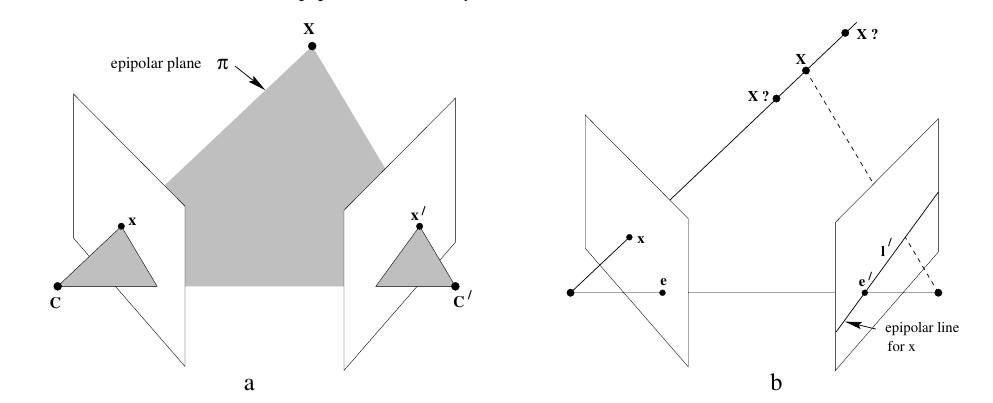
\includegraphics[scale=0.4]{Figs/epipolar.png}
            \caption{Par estéreo.\cite{Zisserman}}
            \label{1}
        \end{figure}

O plano $\pi$, plano epipolar, é delimitado como mostrado na figura 1(a). Pontos em posi\c{c}ões diferentes geram planos, que são sempre rota\c{c}ões em torno da \textit{baseline}, formando o chamado pincel de planos epipolares\cite{Zisserman}. 

\subsection{Matriz fundamental}

A matriz fundamental $F$ obedece a condi\c{c}ão $x'Fx = 0$, sendo $x$ e $x'$ os pontos da direita e da esquerda, respectivamente. $F$ é de rank 2 e possui sete parâmetros: dois para cada epipolo e três da homografia dos planos das imagens \cite{Gary}. Outra propriedade da matriz $F$ é que para todo ponto $x$ sua linha epipolar correspondente é dada por $l^{\prime} = Fx$ \cite{Zisserman}. De forma similar, o epipolo $e^{\prime}$ satisfaz $e^{{\prime}T}(F x) = 0$ \cite{Zisserman}.

\section{Metodologia}

\subsection {Correspondência entre pontos}
A primeira parte do experimento consistiu em achar a correspondência de um ponto da imagem da esquerda, à escolha do usuário, e encontrar o ponto correspondente na imagem da direita. Foram utilizadas imagens da base de dados estéreo de Middleburry\cite{Middle}, que consiste em pares de fotos cujas câmeras estão alinhadas e com a mesma orienta\c{c}ão, ou seja, as linhas epipolares são horizontais. As matrizes de calibra\c{c}ão são dadas na própria base de dados, tendo sido obtidas conforme \cite{Daniel}. Foram consideradas apenas os pares \textit{perfect}. 

Para achar o ponto correspondente na imagem da direita foi utilizado o algoritmo de coeficientes normalizados do OpenCV, cv2.TM\_COEFF\_NORMED\cite{cv}. O usuário digita o tamanho da janela de template que será usada no algoritmo, instanciando uma classe \textit{Window} que gera a janela. Como não foi aplicado nenhum \textit{padding}, pontos muito próximos à borda são considerados inválidos. O resultado dado pelo algoritmo é uma nova coordenada na imagem da direita que corresponde à da esquerda. Um quadrado verde do tamanho da janela é desenhado e mostrado na tela, bem como as coordenadas da imagem da direita.

Tendo os dados da proje\c{c}ão de um mesmo ponto em duas imagens bem como a distância focal e a \textit{baseline} das câmeras, é possível calcular a profundidade para todos os pontos que possuem correspondência, bem como as coordenadas $X$ e $Y$ do mundo real. 

\subsection{Mapa de disparidade e de profundidade}

\subsubsection{Base de dados da Middleburry}

Criar o mapa de disparidade é uma tarefa que envolve uma manipulação algébrica para obter
a matriz fundamental do par estéreo.  Entretanto como a base de dados de Middleburry já
trás imagens retificadas, tais contas serão simplificadas.  O algoritmo do OpenCV utilizado
foi o stereoSGBM\_matcher para a correspondência estéreo e cv2.createDisparityWLSFilter para a cria\c{c}ão do mapa de disparidade. O algoritmo SGBM (\textit{Semi-Global Block Matching} utiliza como principais parâmetros o tamanho de janela, disparidade mínima e número de disparidades. Pontos que não possuem correspondência são por padrão colocados como 0. Nesse caso, é fácil notar que apenas pontos na faixa de $([0, heigth],[0, baseline])$ não terão correspondência, já que as linhas epipolares são horizontais. Assim é possível identificar se um ponto que tem valor de disparidade nulo é um ponto de não correspondência ou se a disparidade é de fato zero naquele ponto.


\section{Resultados e Análise}

Clicando no ponto $(434, 337)$, o algoritmo de correspondência para uma janela de tamanho 11 px foi o ponto $(389, 337)$. Nota-se que a coordenada x permanece inalterada, o que indica que de fato não há altera\c{c}ão na altura correspondente. O algoritmo funciona bem com janelas maiores (aproximadamente 55 px). Um possível motivo para isso é que janelas menores têm maiores chances de encontrarem bordas ou outras features que destaquem a região. Áreas "lisas" como paredes ou com luz uniforme tendem a errar na correspondência. As imagens resultantes para um clique são mostradas nas figuras 2 e 3. As coordenadas do mundo para o mesmo ponto foram dadas por $(618.44, 411.06, 153.1)$ mm.

\begin{figure}[htbp]
  \centering
  \begin{minipage}[b]{0.44\textwidth}
    \includegraphics[width=\textwidth]{Figs/EsquerdaPiano.png}
    \caption{Imagem da esquerda}
  \end{minipage}
  \hspace{2.4mm}
  \begin{minipage}[b]{0.44\textwidth}
    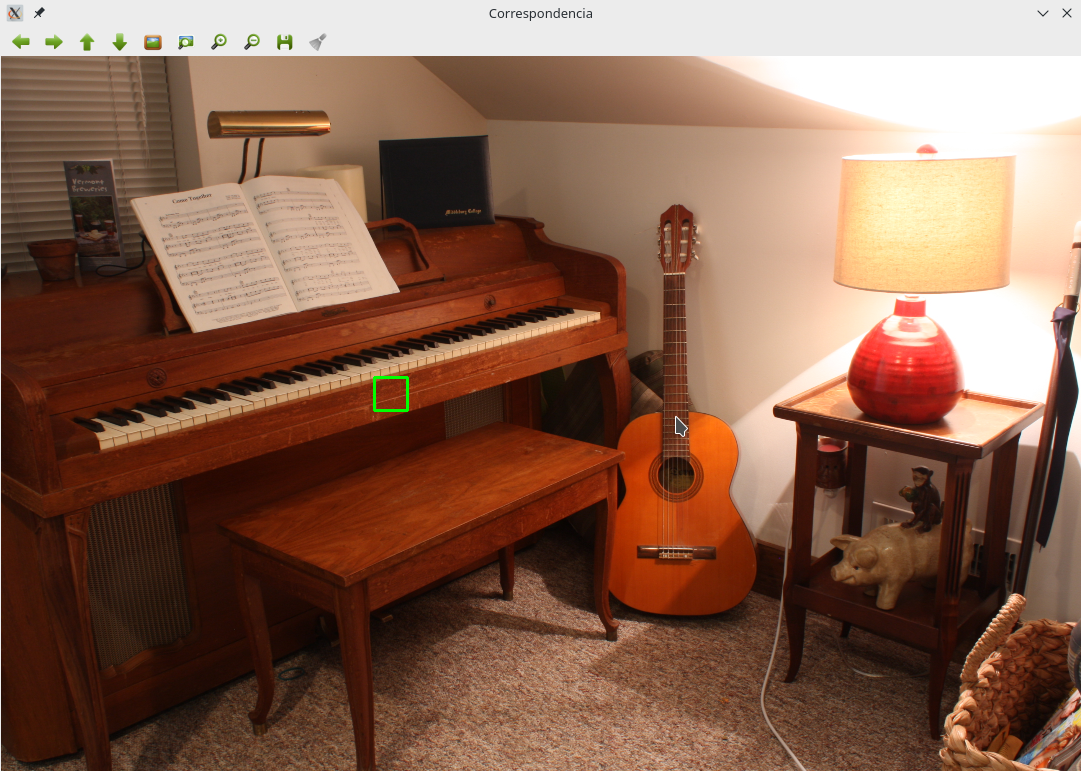
\includegraphics[width=\textwidth]{Figs/CorrespPiano.png}
    \caption{Imagem da direita}
  \end{minipage}
\end{figure}

O mapa de disparidade para o cenário piano e playroom estão exibidos nas figuras 4 e 5, respectivamente. O mapa de profundidade foi obtido utilizando os pontos Z das coordenadas do mundo transformados pra unsigned int de 8 bits, resultando nas figuras 6 e 7. As distâncias foram normalizadas de acordo com a maior distância possível em cada imagem. Por ser uma imagem com pouca profundidade máxima muito baixa, a imagem playroom ficou muito escura e com muitos pontos marcados em branco, o que possivelmente indica que a normaliza\c{c}ão foi prejudicada.

\begin{figure}[htbp]
            \centering
            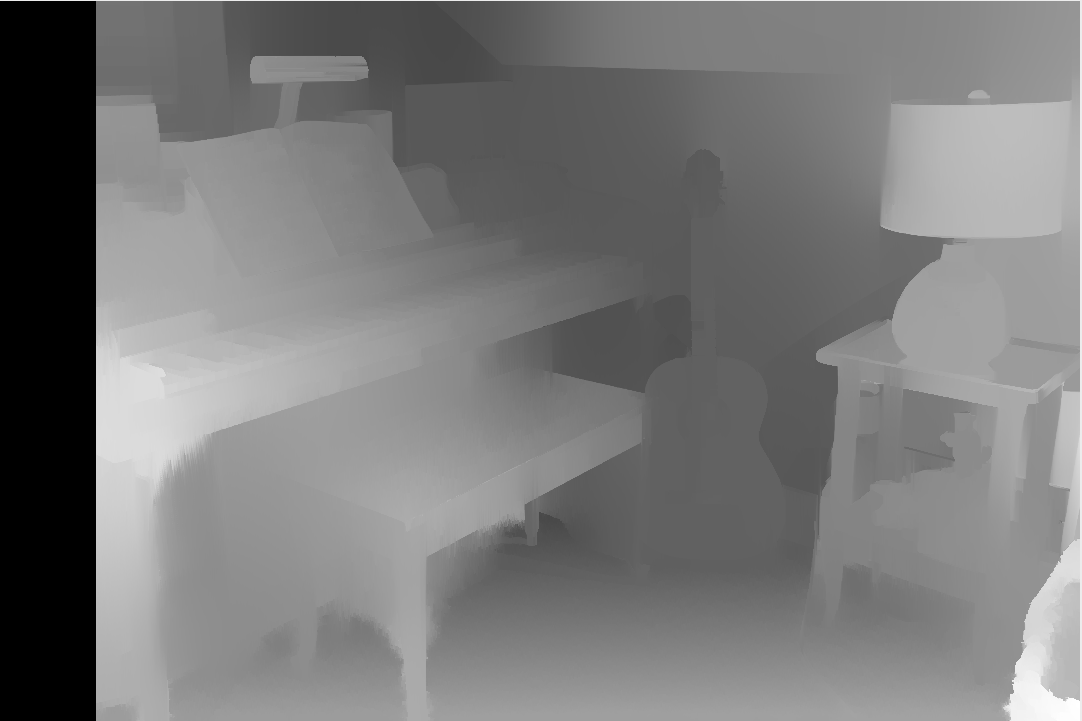
\includegraphics[scale=0.3]{Figs/disppiano.png}
            \caption{Mapa de disparidade - Piano (perfect)}
            \label{1}
        \end{figure}
        
\begin{figure}[htbp]
            \centering
            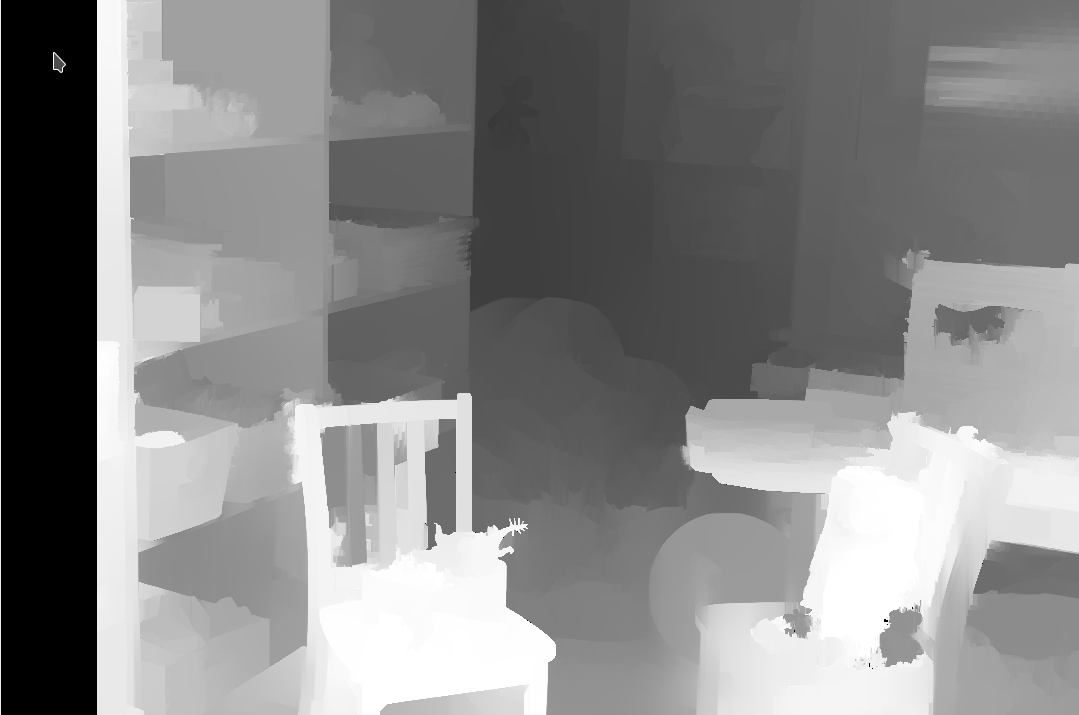
\includegraphics[scale=0.3]{Figs/dispplay.png}
            \caption{Mapa de disparidade - Playroom (perfect)}
            \label{1}
        \end{figure}
        
\begin{figure}[htbp]
            \centering
            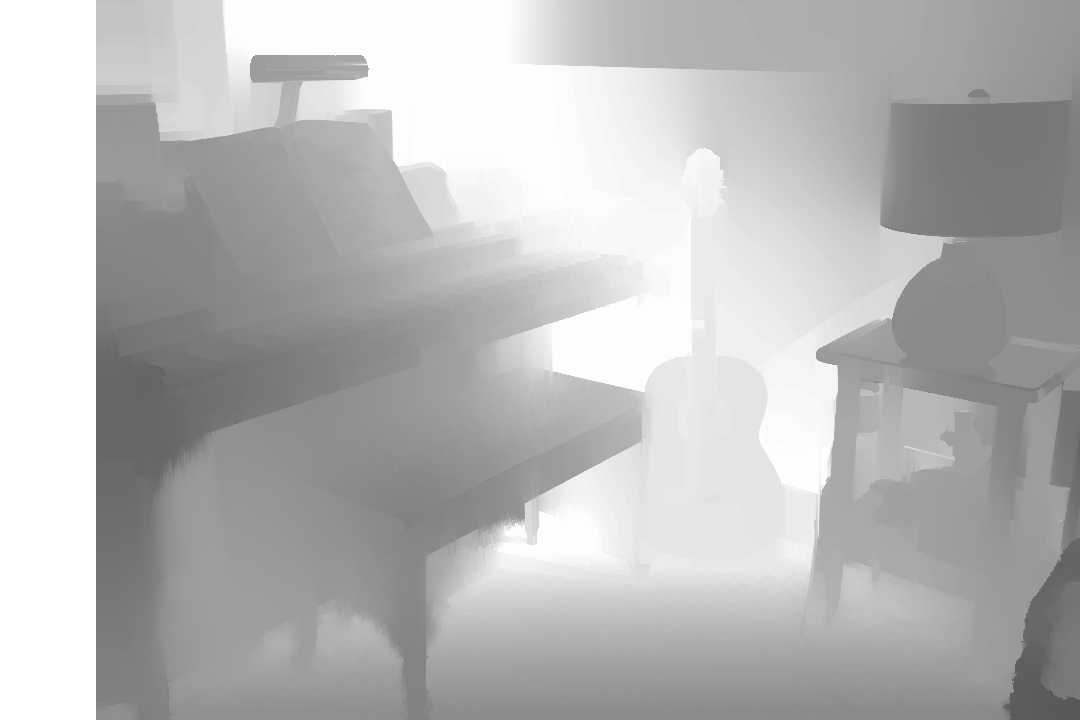
\includegraphics[scale=0.25]{Figs/profundidade.png}
            \caption{Mapa de profundidade - Piano (perfect)}
            \label{1}
        \end{figure}
        
\begin{figure}[htbp]
            \centering
            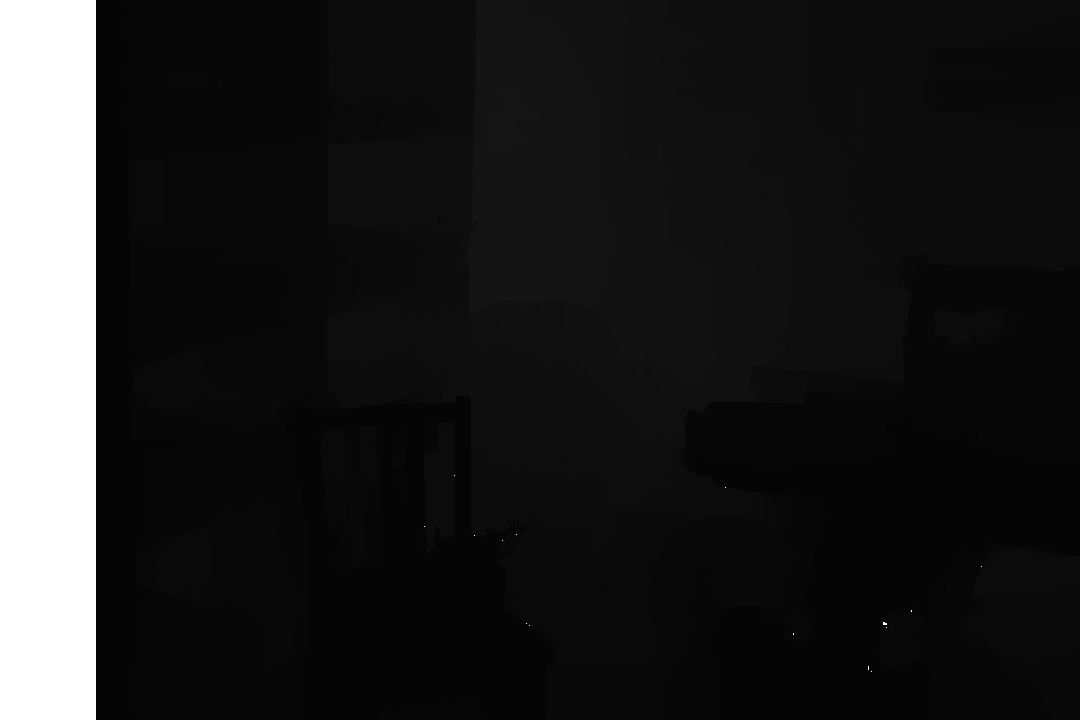
\includegraphics[scale=0.25]{Figs/profundidade1.png}
            \caption{Mapa de profundidade - Playroom (perfect)}
            \label{1}
        \end{figure}

\newpage

        
\section{Conclusão}

O algoritmo de correspondência entre imagens estéreo funciona melhor com janelas menores, o que sugere que quanto mais informa\c{c}ão a janela tiver melhor a chance de acerto. As disparidades tiveram muita distor\c{c}ão, o que sugere que possivelmente a calibra\c{c}ão realizada pelos parâmetros não foi perfeita. A imagem do playroom é interessante, pois a profundidade de todos os pontos é relativamente parecida, o que tornou o mapa de profundidade muito escuro, dificilmente sendo possível identificar alguma forma.

%-------------------------------------------------------------------------

\bibliography{refs}
\end{document}
